\documentclass[a4paper]{article}

\usepackage[english]{babel}
\usepackage[utf8]{inputenc}
\usepackage{amsmath}
\usepackage{graphicx}
\usepackage[colorinlistoftodos]{todonotes}
\usepackage{float}

\title{Bubble Beam - Assignment 2}

\author{
    Bavdaz, Luka\\
    \texttt{4228561}
    \and
    Clark, Liam\\
    \texttt{4303423}
    \and
    Gmelig Meyling, Jan-Willem\\
    \texttt{4305167}
    \and
    Hoek, Leon\\
    \texttt{4021606}
    \and
    Smulders, Sam\\
    \texttt{4225007}
}

\date{\today}

\begin{document}
\maketitle

\section{Simple Logging}

\subsection{Logger implementation}
The logger is successfully implemented and committed.

\subsection{Analysis and design phases}
The documents used during the analysis and design phases of the logger can be found in the folder Assignment\_2\_logger\_analysis\_desing within the report folder.

\section{Design patterns}

\subsection{Iterator}
We used the iterator pattern to go over all the bubbles in a BubbleMesh. This is for example used to draw all the bubbles in a BubbleMesh.

We added methods for BubbleMesh to create an iterator for the BubbleMesh. These methods each create a new instances of the BubbleMeshIterator, which creates a list of all bubbles of a row in the BubbleMesh that require iterating. To iterate through the entire mesh, multiple iterators are used. Our BubbleMeshIterator has a method to remove the next Bubble on the list and return it and has a method to tell if the list is empty or is not.

\subsubsection{Natural language description}

\subsubsection{Class diagram}
\begin{figure}[H]
\centering
    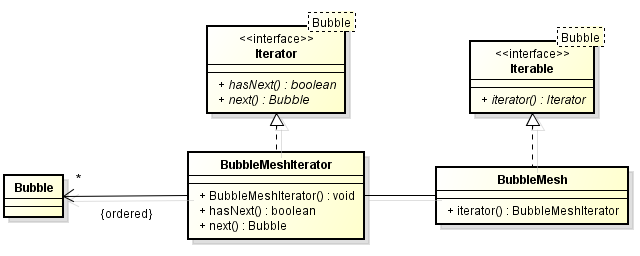
\includegraphics[width=1.0\textwidth]{iterator_class_diagram_v2.PNG}
    \caption{\label{fig:class_iterator} The class diagram for the implemented iterator pattern}
\end{figure}

\subsubsection{Sequence diagram}
\begin{figure}[H]
\centering
    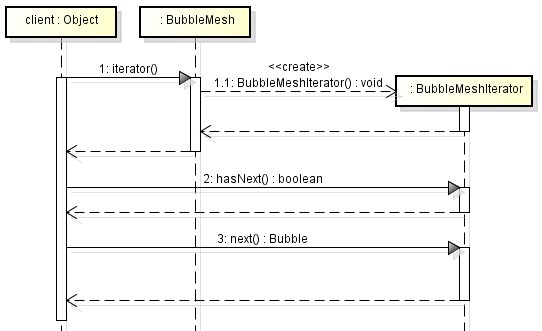
\includegraphics[width=1.0\textwidth]{iterator_sequence_diagram.PNG}
    \caption{\label{fig:sequence_iterator} The sequence diagram for the implemented iterator pattern}
\end{figure}

\subsection{Observer}

\subsubsection{Description of the Observer Pattern}

We needed a nice way to encapsulate the GUI code and the logic behind our model and at the same time make the code more testable. We decided to make the Cannon class simply draw the cannon according to a model. 

We decided on the workflow displayed in figure  \ref{fig:sequence_observer}. The Cannon and the Controller are very loosely coupled through the model. The Cannon draw according to the data from the model and doesn’t need any logic for controlling it. This also makes testing the class easier since it now has just a single behaviour (drawing) instead of multiple behaviours of drawing and controlling. 

We ran into trouble when the model needed to be able to shoot. This is an action and that can’t be done through just observer you need an ActionListener for this. For that purpose in the AbstractCannonController listeners are bound to the model slightly tightening the coupling between them. This isn’t perfect but it will work for now and it’s still a great we eventually implemented it following the model in figure \ref{fig:class_observer}.

\subsubsection{Class diagram}
\begin{figure}[H]
    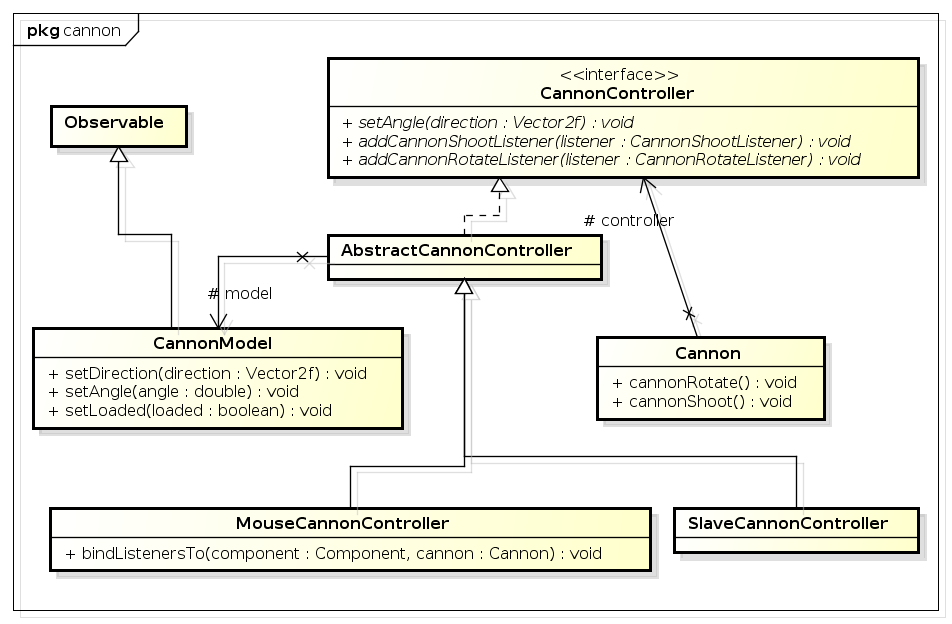
\includegraphics[width=1.0\textwidth]{Class_Diagram_Observer_Pattern.png}
    \caption{\label{fig:class_observer} The class diagram for the implemented observer pattern}
\end{figure}

\subsubsection{Sequence diagram}
\begin{figure}[H]
    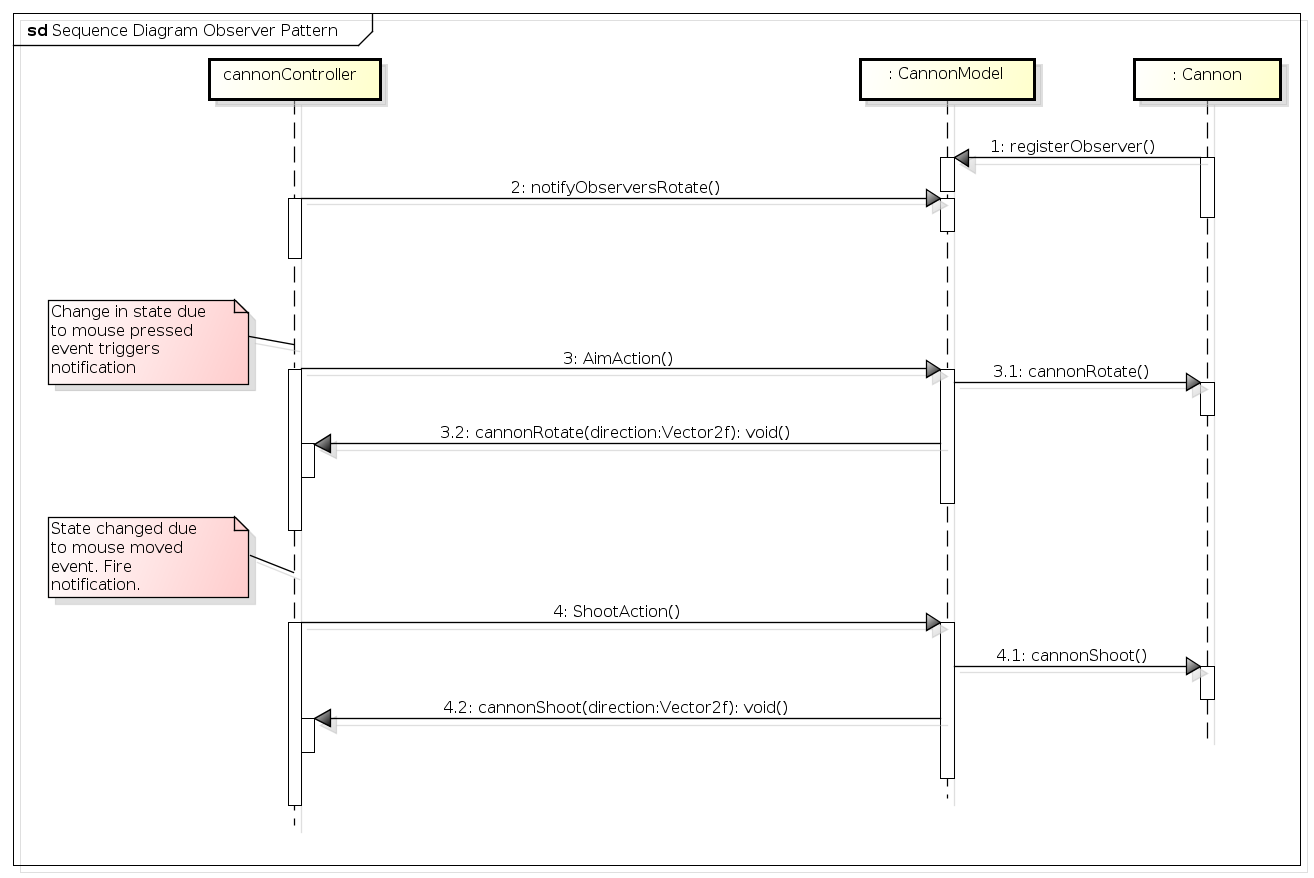
\includegraphics[width=1.0\textwidth]{Sequence_Diagram_Observer_Pattern.png}
    \caption{\label{fig:sequence_observer} The sequence diagram for the implemented observer pattern}
\end{figure}

\subsection{Strategy pattern}

\subsubsection{Natural language description}

Using the Stratagy patern makes it possible to add new behaviour without changing other classes. The reason for implementing this pattern was to make the program more flexible, because the behaviours are loosly coupled. For example, we could implement an teleportation bubble that teleports the first movingBubbles colliding with it, after which the behaviour changes. To achieve this, a new behaviour for teleporting has to be added.

A SnapBehaviour interface was introduced, as displayed in figure \ref{fig:class_strategy}, which is implemented in the subclasses, each representing a type of different behaviour. In this case, the SnapToClosest algorithm returns the closest PlaceholderBubble using a search method, while the SnapToSelf returns itself. The AbstractBubble has an instance of the behaviour, which is set in the constructor depending on the subclass.

The SnapClosest algorithm is implemented by the ColouredBubble class, since it takes up a bubble spot where a new bubble cannot simply be placed without removing a bubble. The SnapToClosest algorithm will also be used by every new class at which a new bubble arrives but cannot stay. The SnapToSelf algorithm is used by the BubblePlaceholder class, because a newly arriving bubble can take its place.

\subsubsection{Class diagram}
\begin{figure}[H]
    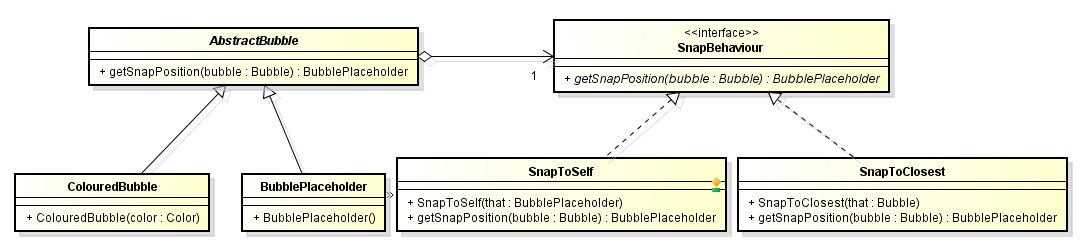
\includegraphics[width=1.0\textwidth]{uml_strategy.PNG}
    \caption{\label{fig:class_strategy} The class diagram for the implemented strategy pattern}
\end{figure}

\subsubsection{Sequence diagrams}
The sequence diagrams \ref{fig:sequence_strategy1} and \ref{fig:sequence_strategy2} show how the pattern works dynamically in our code.
\begin{figure}[H]
    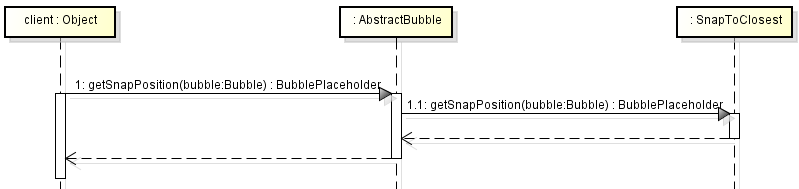
\includegraphics[width=1.0\textwidth]{sequence_strategy_1.PNG}
    \caption{\label{fig:sequence_strategy1} The sequence diagram for the implemented strategy pattern for the SnapToClosest behaviour}
\end{figure}
\begin{figure}[H]
    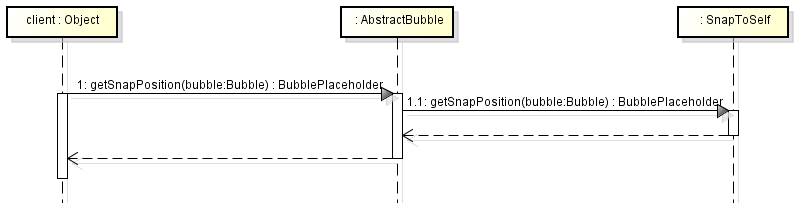
\includegraphics[width=1.0\textwidth]{sequence_strategy_2.PNG}
    \caption{\label{fig:sequence_strategy2} The sequence diagram for the implemented strategy pattern for the SnapToSelf behaviour}
\end{figure}

\section{State pattern}

\subsection{Natural language description}
The state design pattern was implemented to remove the conditional statements regarding the possibility of shooting and make the code more open to extension. 

For every cannon state there is a seperate class that implements the CannonState interface. The cannon state of a cannon is tracked by a CannonController. This CannonController calls the shoot method, every time the CanonController wants to shoot. The CannonState determines if shooting actually occurs. If. tI dthe cannoesn controller uses shoot on a CannonLoadedState, the CannonState notifys all the listeners of the CannonController. If the cannon is in the CannonShootState, the cannon can't shoot, and has to wait till the CannonState is set back to the CannonLoadedState. This is done by the GameController, once a moving bubble hits a bubble from the bubble mesh.
\subsection{Class diagram}

\begin{figure}[H]
    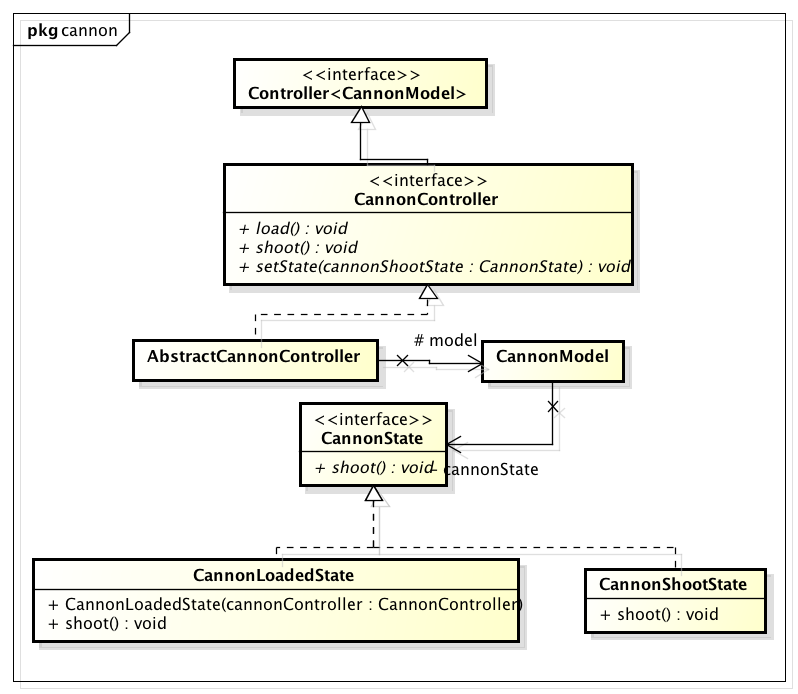
\includegraphics[width=1.0\textwidth]{CannonStateDiagram.png}
    \caption{\label{fig:class_state} The class diagram for the implemented state pattern for the Cannonload behaviour}
\end{figure}

\subsection{Sequence diagrams}
\begin{figure}[H]
  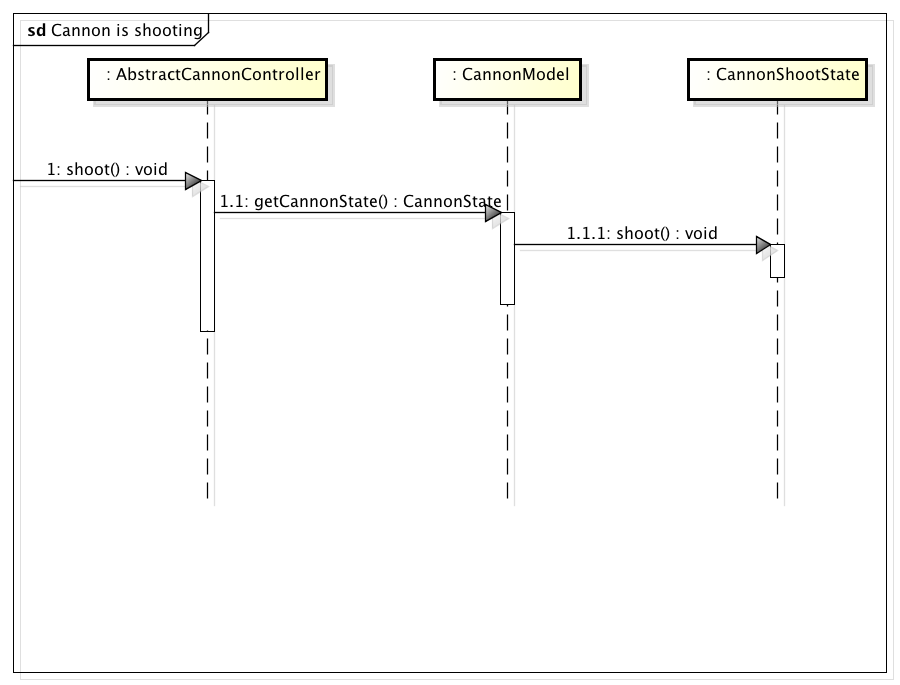
\includegraphics[width=1.0\textwidth]{CannonShoot_state_Sequence_Diagram.png}
    \caption{\label{fig:sequence_state1} The sequence diagram for the implemented state pattern for the Cannonload behaviour}
\end{figure}

\begin{figure}[H]
 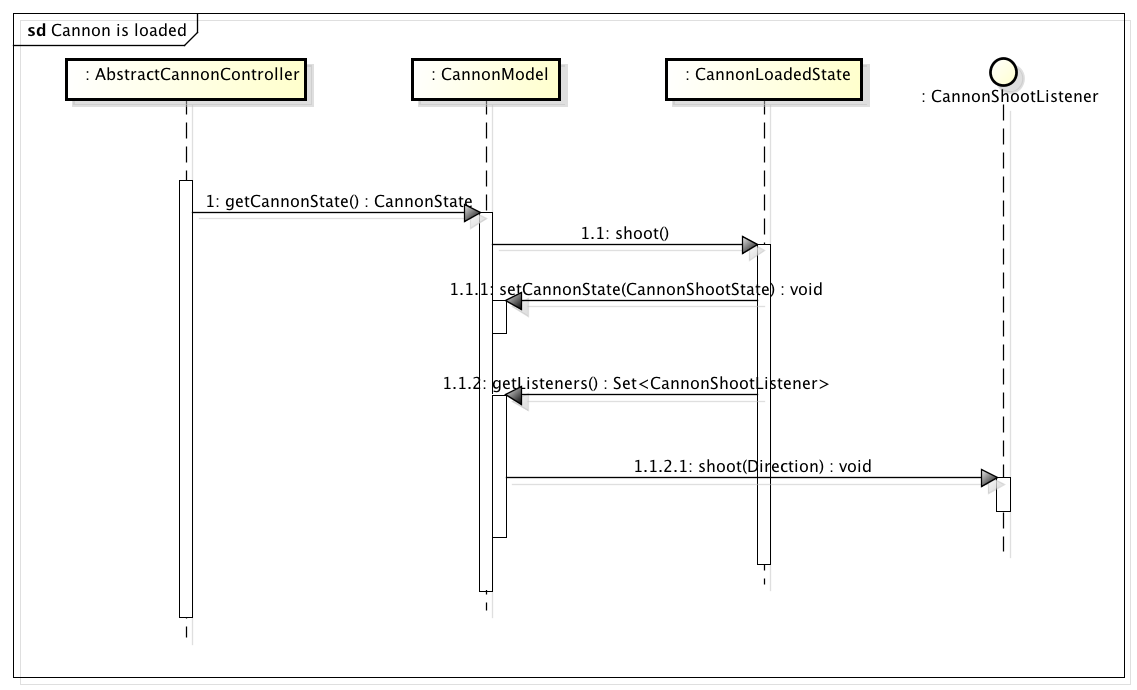
\includegraphics[width=1.0\textwidth]{CannonLoaded_Sequence_Diagram.png}
	\caption{\label{fig:sequence_state2} The class diagram for the implemented state pattern for the Cannonload behaviour}
\end{figure}

\end{document}